%Olli
\section{Optimierung}\label{Opt}\label{olli:optimierung}
In diesem Teil der Arbeit wird die Optimierung der Kraftwerksverteilung
erl�utert. Dies wird auf der Seite des Clients ausgef�hrt --- dadurch wird die
Komplexit�t des Algorithmus reduziert, da die Daten des Servers nicht mit denen 
des Clients synchronisiert werden m�ssen. Aus Spielgr�nden wurde entschieden, 
dass sich der Spieler nicht selbst um die Optimierung der Kraftwerke k�mmern 
muss, sondern dass die Optimierung mithilfe des Simplexalgorithmus durchgef�hrt 
wird, da die Kraftwerksverteilung durch ein lineares Optimierungsproblem
formuliert werden kann (\seCite{vgl.}{}{holey}).

Zun�chst stellt dies das folgende Problem dar: \\
$k$ Kraftwerke mit einer Produktion von $k_i$ haben je $x$ Verbindungen zu $s$
St�dten mit je $y$ Verbindungen, einem Preis $p$ und einem Bedarf $n$. Dabei wird eine Verbindung nur gebildet,
wenn der Spieler mit der jeweiligen Stadt einen Vertrag besitzt und das
Kraftwerk  h�chstens drei Felder von der Stadt entfernt ist. So k�nnte 
beispielsweise folgendes Optimierungsproblem entstehen:

%Bild Optimierung
\begin{figure}[H]
\centering
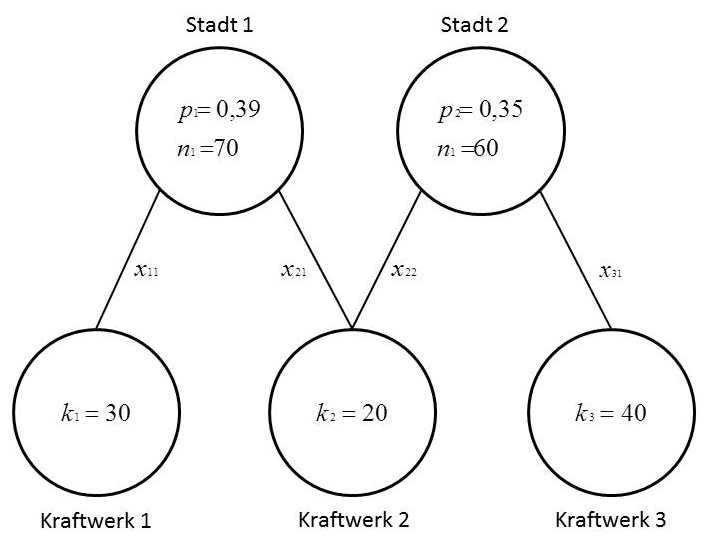
\includegraphics[width=0.85\textwidth]{se-wa-jpg/optimizing}
\caption{Beispiel Optimierungsproblem}
\label{Beispielproblem}
\end{figure}

Nach dem Simplexalgorithmus m�ssen f�r dieses Problem nun die Zielfunktion und
die Nebenbedingungen aufgestellt werden. Die Zielfunktion $z$ ist durch die 
Maximierung des Umsatzes gegeben. Dabei ist $p_i$ der Preis der Stadt $i$,
$k_j$ die maximale Produktion des Kraftwerkes $j$ und $y_j$ die Verbindung
zwischen der Stadt und dem Kraftwerk.

\begin{align*}
z &= \sum\limits_{i=1}^s p_i * \sum\limits_{j=1}^y y_j * k_j \\
  &= 0.39 (x_{11} * 30 + x_{21} * 20) + 0.35 (x_{22} * 20 + x_{31} * 40)
\end{align*}

Als n�chstes wird f�r jedes Kraftwerk eine Nebenbedingung erstellt. Die
Verteilung der Produktion eines Kraftwerkes ist durch mehrere
Variablen $x_i$ gegeben (pro Kraftwerkverbindung eine).
Addiert d�rfen diese h�chstens $1$ sein, damit das Kraftwerk nicht mehr auf die
Verbindungen verteilt, als es eigentlich maximal produzieren kann:

\begin{align*}
g: &\sum\limits_{i=1}^x x_i &\leq 1 \\
g_1: &x_{11} &\leq 1 \\
g_2: &x_{21} + x_{22} &\leq 1 \\
g_3: &x_{31} &\leq 1
\end{align*}

Anschlie�end wird f�r jede Stadt eine Nebenbedingung erstellt, in der der
maximale Bedarf $n$ der Stadt gepr�ft wird. $y$ ist hier die Anzahl der Verbindungen der
Stadt und $k_j$ die Produktion des Kraftwerkes $j$:

\begin{align*}
g: \sum\limits_{j=1}^y y_j * k_j \leq n \\
g_4: 30x_{11} + 20x_{21} \leq 50 \\
g_5: 20x_{22} + 40x_{31} \leq 60
\end{align*}

Danach werden die Zielfunktion und die Nebenbedingungen in die Normalform
gebracht. In diesem Fall werden in den Nebenbedingungen nur Schl�pfvariablen
angelegt und als Startl�sung die Kraftwerksverbindungsvariablen $x_i = 0$
gesetzt. Darauffolgend werden nach dem Simplexalgorithmus die Daten in eine
Matrix eingef�gt:

\begin{align*}
\begin{array}{ c | c | c | c | c | c | c | c | c | c | c }
BV & x_{11} & x_{21} & x_{22} & x_{31} & s_1 & s_2 & s_3 & s_4 & s_5 & b \\
\hline
s_1 & 1 & 0 & 0 & 0 & 1 & 0 & 0 & 0 & 0 & 1 \\ 
s_2 & 0 & 1 & 1 & 0 & 0 & 1 & 0 & 0 & 0 & 1 \\
s_3 & 0 & 0 & 0 & 1 & 0 & 0 & 1 & 0 & 0 & 1 \\
s_4 & 30 & 20 & 0 & 0 & 0 & 0 & 0 & 1 & 0 & 50 \\
s_5 & 0 & 0 & 20 & 40 & 0 & 0 & 0 & 0 & 1 & 60 \\
\hline
z & -0.39*30 & -0.39*20 & -0.35*20 & -0.35*40 & 0 & 0 & 0 & 0 & 0 & 0
\end{array}
\end{align*}

Nach mehreren Iterationsschritten zeigt sich folgende L�sung als optimal:

\begin{align*}
x_{11} &= 1 & s_1 &= 0 \\
x_{21} &= 1 & s_2 &= 0 \\
x_{22} &= 0 & s_3 &= 0 \\
x_{31} &= 1 & s_4 &= 0 \\
& & s_5 &= 20
\end{align*}

Die Stadt $s_1$ wird aufgrund des h�heren Preises vom Kraftwerk $k_2$ bevorzugt
und wird deswegen �ber die Verbindung $x_{21} = 1$ beliefert. $x_{22} = 0$
bedeutet, dass $k_2$ zwar an Stadt $s_2$ liefern k�nnte, es aber nicht macht. Die
Schl�pfvariablen $s_{1\ldots3} = 0$ bedeutet, dass alle Kraftwerke ihre
komplette Produktion nutzen. Zuletzt bedeutet $s_4 = 0$, dass der Bedarf von
Stadt $s_1$ komplett gef�llt wird und $s_5 = 20$, dass der Stadt $s_2$ noch
$20$ Einheiten fehlen.



